% ------------------------------------------------------------------
\documentclass[aps,prl,twocolumn,]{revtex4}  % for review and submission

%\documentclass[aps,prl]{revtex4}  % for double-spaced preprint
\usepackage{graphicx}  % needed for figures
\usepackage{dcolumn}   % needed for some tables
\usepackage{bm}        % for math
\usepackage{amssymb}   % for math
\usepackage{color} 



\usepackage{amsmath}

%\usepackage{geometry}                % See geometry.pdf to learn the layout options. There are lots.
%\geometry{letterpaper}                   % ... or a4paper or a5paper or ... 
%\geometry{landscape}                % Activate for for rotated page geometry
%\usepackage[parfill]{parskip}    % Activate to begin paragraphs with an empty line rather than an indent
%\usepackage{amssymb}
\usepackage{epstopdf}
\DeclareGraphicsRule{.tif}{png}{.png}{`convert #1 `dirname #1`/`basename #1 .tif`.png}

\usepackage{bm}       % for math
\usepackage{amsmath}
%\usepackage{cite}     % Collapses refs at the price of losing links
\usepackage{cancel}
%\usepackage{dblfloatfix}



\newcommand{\bee}{\begin{equation}}
\newcommand{\ee}{\end{equation}}
\newcommand{\beea}{\begin{eqnarray}}
\newcommand{\eea}{\end{eqnarray}}
\newcommand{\be}{\ensuremath{\beta} }
\newcommand{\cO}{\ensuremath{\mathcal O} }
\newcommand{\X}{\ensuremath{\!\times\!} }
\newcommand{\lsim}{\ensuremath{\lesssim} }
\newcommand{\Sb}{\ensuremath{\cancel{S^4}} }
\newcommand{\refcite}[1]{Ref.~\cite{#1}}
\newcommand{\eq}[1]{Eq.~\ref{#1}}
\newcommand{\fig}[1]{Fig.~\ref{#1}}
\newcommand{\TODO}[1]{\textcolor{red}{{\bf #1}}}
\newcommand{\mysection}[1]{\vspace{-12 pt}\section{#1}\vspace{-6 pt}}
% ------------------------------------------------------------------

\begin{document}
% ------------------------------------------------------------------
\title{Finite size scaling of conformal theories in the presence of a near-marginal operator}


\author{Anqi~Cheng}
\affiliation{Department of Physics, University of Colorado, Boulder, CO 80309, USA}
\author{Anna~Hasenfratz}
\affiliation{Department of Physics, University of Colorado, Boulder, CO 80309, USA}
\author{Yuzhi~Liu}
\affiliation{Department of Physics, University of Colorado, Boulder, CO 80309, USA}
\author{Gregory Petropoulos}
\affiliation{Department of Physics, University of Colorado, Boulder, CO 80309, USA}
\author{David~Schaich}
\affiliation{Department of Physics, University of Colorado, Boulder, CO 80309, USA}
\email{anna@eotvos.colorado.edu}

\begin{abstract}
Understanding the non-perturbative behavior of strongly coupled gauge-fermion systems  are essential for many BSM theories  but the  slowly evolving gauge coupling  makes  numerical investigations of these models challenging. We consider finite size scaling and show that this  often used technique leads to inconsistent results if the near-marginal gauge coupling is neglected. When the corrections are included the results become consistent not only between different operators but between different gauge couplings, even when  data obtained using different lattice actions are combined. Or results indicate that the SU(3) 12-fermion system is conformal with mass anomalous dimension $\gamma_m=0.xx(xx)$. We also consider the finite size scaling  of the 8-flavor system using available data from several collaborations. The results could be consistent both with conformal and chirally broken infrared dynamics, suggesting  that significantly larger volumes are needed to study the infrared dynamics of this system. 
\end{abstract}

\maketitle


% ------------------------------------------------------------------



% ------------------------------------------------------------------

%\section{Introduction}

Strongly coupled gauge-fermion systems near the conformal window are   candidates to describe the dynamics of electroweak symmetry breaking and beyond-Standard Model physics. A walking  gauge coupling  with large anomalous dimension can give rise to an enhanced fermion condensate,  while the weakly broken conformal symmetry results in a light dilaton that could play the role of the Higgs boson. While the  non-perturbative properties of these systems are well suited to lattice studies,   standard lattice methods are frequently not efficient to investigate the infrared properties of near-conformal systems. The problems are mainly due to  the nearly marginal "walking" nature of the irrelevant gauge coupling. In this paper we investigate finite size scaling, a well established method to predict critical scaling exponents in the vicinity of fixed points with one relevant operator, and show that it is essential to take into account the effect of the nearly marginal gauge coupling to obtain consistent results. 

We concentrate on the SU(3) gauge model with 12 fundamental fermions,
a controversial system.
Several groups have studied the infrared properties of this model using different methods and different lattice actions, arriving at contradictory conclusions regarding its IR dynamics.
(For a limited set of references see Refs.~\cite{Appelquist:2009ty, Deuzeman:2009mh, Hasenfratz:2011xn, Fodor:2011tu, Appelquist:2011dp,DeGrand:2011cu, Cheng:2011ic, Cheng:2013eu, Fodor:2012uw, Fodor:2012et,  Aoki:2012eq, Aoki:2013pca, Itou:2012qn, Lin:2012iw, Jin:2012dw} .) In particular finite size scaling was considered in \refcite{Fodor:2011tu,Appelquist:2011dp,DeGrand:2011cu,Fodor:2012et,Aoki:2012eq}. Inconsistencies of the scaling exponent as predicted by different operators lead some authors to strongly question the conformal  behavior of this model.

We investigate this system at several gauge coupling values, and  also analyze the published data of the Lattice Higgs (LHC) and LatKMI collaborations~\cite{Fodor:2011tu,Aoki:2012eq}. We develop a simple  formalism that  takes into account the effect of the nearly marginal gauge coupling and find consistent results for different operators  when several gauge couplings are combined, and even when different lattice actions are considered together. Our results suggest conformal infrared dynamics. The fit parameters suggest that at least some of the data are in the strong coupling region relative to the apparent infrared fixed point, further supporting conformal dynamics. The predicted mass anomalous dimension, $\gamma_m=0.20(xx)$, is consistent with results we obtained from the scaling of the Dirac operator spectral density. Preliminary results of our investigations have been reported in \refcite{Hasenfratz:2013eka}.

To further test our finite size scaling approach we analyze the available data for $N_f=8$ fermion flavors  from the LatKMI group~\cite{Aoki:2013xza} and  the USBSM collaboration~\cite{Schaich:2013eba}, combined with our own smaller data set. We find that all the data are consistent with  conformal finite size scaling  with scaling exponent $\gamma_m=0.xx(xx)$. However this result could be consistent both with conformal and  chirally broken  infrared behavior as the data appear to be in the  weak coupling regime of a slowly walking system where available lattice volumes are insufficient to distinguish the two  dynamics.




%%%%%%%%%%%%%%%%%%%%%%%%%%%%%%%%%%
\begin{figure*}[tb]
\centering
  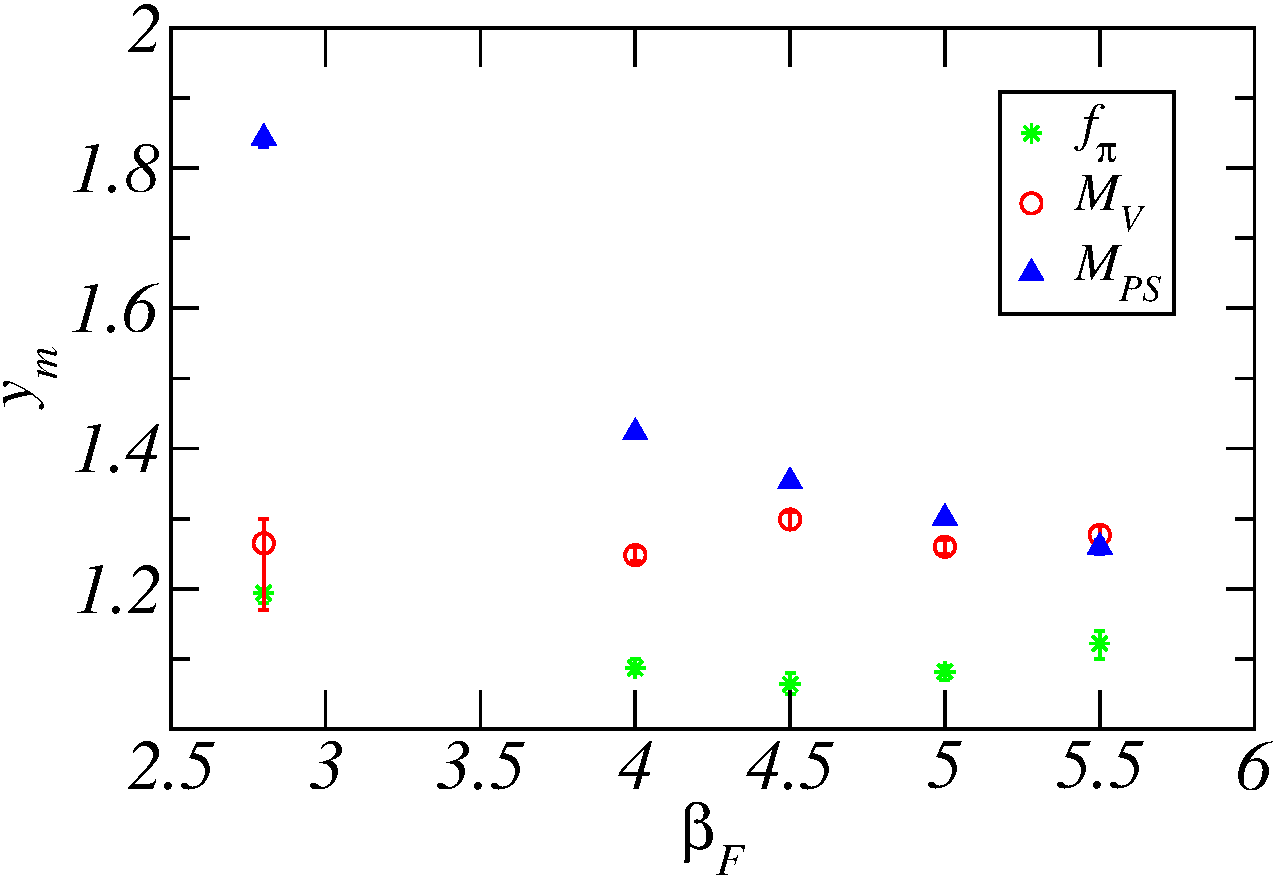
\includegraphics[width=0.45\linewidth]{ym_c0} \hfill
  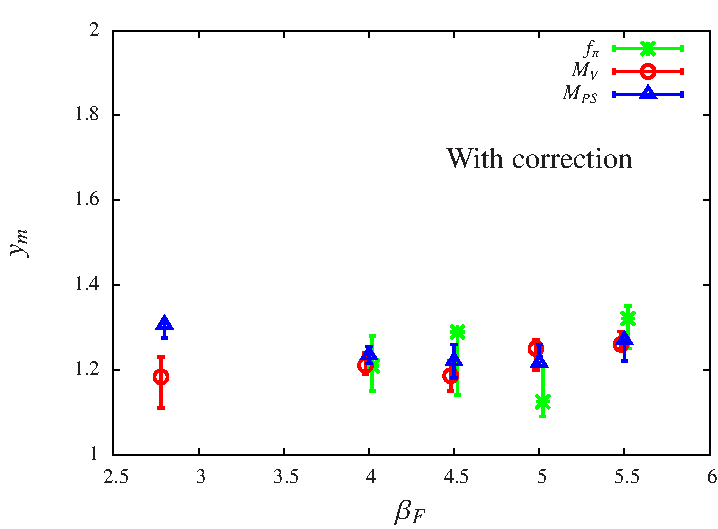
\includegraphics[width=0.45\linewidth]{ym}
   \caption{\label{fig:scaling_exp} The scaling dimension $y_m$ predicted by finite size scaling, as a function of the gauge coupling $\beta_F$ for the pseudoscalar (blue triangles), vector (red circles) and $f_\pi$ (green $\times$s).  Left: fits including only the relevant mass operator (~\protect\eq{eq:leading_fss}).  Right: fits including both the relevant operator and leading irrelevant corrections (\protect\eq{eq:corrected}) with $y_0=-0.36$ fixed at the two-loop value.}
 \end{figure*}
%%%%%%%%%%%%%%%%%%%%%%%%%%%%%%%%%


% ------------------------------------------------------------------
\section{Finite size scaling}
Finite size scaling is a well understood technique in statistical physics.
Its derivation is easiest using renormalization group analysis and has been reviewed recently in connection with infrared conformal systems \cite{DeGrand:2009mt, DelDebbio:2010ze,DelDebbio:2013qta}.
Here we summarize only the steps relevant for the scaling of physical quantities ``$M_H$'' with mass (engineering) dimension $[M_H] = 1$.

For concreteness consider a system with one relevant operator, denoted by $m$, that has a scaling dimension $y_m > 0$.
All other operators, denoted by $g_i$, are irrelevant with scaling exponents $y_i < 0$.
Renormalization group arguments predict that in a finite spatial volume $L^3$, $M_H$ depends only on specific combinations of the couplings, and can be written as
\begin{equation}
  \label{eq:general}
  M_H = L^{-1} f\left(x, g_i m^{-y_i / y_m}\right),
\end{equation}
where $x \equiv L m^{1 / y_m}$.
In the critical $m\to 0$ limit, $g_i m^{-y_i / y_m} \to 0$ and we find the familiar finite-size scaling formula
\begin{equation}
\label{eq:leading_fss}
  M_H = L^{-1} f_H(x),
\end{equation}
where $f_H(x)$ is an arbitrary but unique scaling function that
depends on the observable $M_H$. The exponent $y_m$  is universal, characteristic of the corresponding fixed point.

If one of the irrelevant operators, let's say $g_0$, is nearly marginal with scaling exponent $y_0 \lsim 0$, the term $g_0 m^{-y_0 / y_m}$ can remain significant and has to be included in the scaling analysis.
This leads to the modified finite-size scaling formula
\begin{equation}
  M_H = L^{-1} f\left(x, g_0 m^{\omega}\right),
\end{equation}
where $\omega \equiv -y_0 / y_m \gtrsim 0$.
The scaling function $f\left(x, g_0 m^{\omega}\right)$ is analytic even at the fixed point, and can be expanded as
\begin{equation}
  \label{eq:expansion}
  L M_H = F_H(x)\left\{1 + g_0 m^{\omega} G_H(x) + \cO\left(g_0^2 m^{2\omega}\right)\right\}.
\end{equation}
The first term is the usual finite-size scaling expression; the second term accounts for leading corrections to scaling due to the nearly-marginal $g_0$ coupling.


In the limit $x \to 0$, both $F_H(x)$ and $G_H(x)$ approach finite constants.
In the infinite-volume limit, with small but fixed $m$, $F_H(x)\propto x$ while $G_H(x)$ remains finite.
Our simulations cover a limited range $0.5 \lsim x \lsim 5$, over which we approximate $G_H(x)$ by a constant, $G_H(x) = c_G$, so 
\begin{equation}
  \label{eq:corrected}
  \frac{L M_H}{1 + c_G g_0 m^{\omega}} = F_H(x).
\end{equation}
One can test the validity of this assumption by repeating the analyses using subsets of the data restricted to smaller ranges in $x$.
\eq{eq:corrected} is very similar to the original \eq{eq:leading_fss} and can be fitted similarly.
However, the analysis now involves three parameters: $c_0 \equiv c_G g_0$, $y_0$ and $y_m$.

% ------------------------------------------------------------------




% ------------------------------------------------------------------
\section{Finite size scaling fits}
In our numerical studies we use nHYP smeared staggered fermions with smearing parameters $(0.5,0.5,0.4)$ to ensure the numerical stability of simulations.
Our gauge action contains fundamental and adjoint plaquette terms with $\beta_A/\beta_F=-0.25$ to avoid the potential scaling violation effects known to exist at positive adjoint plaquette coupling.
In \refcite{Cheng:2011ic} we reported on the phase structure and other properties of this action with $N_f=12$ fundamental fermions.

In our previous studies we were able to run simulations in the $m=0$ chiral limit with periodic spatial boundary conditions on volumes as large as $32^3\X64$ at gauge couplings $\beta_F\ge2.8$, up to the single-site shift symmetry broken  \Sb lattice phase~\cite{Hasenfratz:2013uha}.
In the present work we consider gauge couplings on the weak coupling side of the \Sb phase,  $\beta_F=2.8$, 4.0, 4.5, 5.0, 5.5 and 6.0 and volumes $16^3\X32$, $20^3\X40$, $24^3\X48$ and $32^3\X64$.We choose the bare mass in the range $0.005 \leq m \leq 0.12$, requiring that the vector meson mass $M_V < 0.8$.
%Based on our spectrum measurement if this system is conformal, its infrared fixed point is around $\beta_F=5.5-6.0$~\cite{Hasenfratz:2013eka}.



Two loop perturbation theory predicts that the 12 flavor system is conformal with scaling exponent $y_m=1.45$ and leading irrelevant exponent $y_0=-0.36$. We start with the  finite size scaling analysis  using the usual form of \eq{eq:leading_fss}, ignoring the effect of the near-marginal gauge coupling. We consider each operator and $\beta_F$ data set independently and fit the $M_H L$ versus $x$ with two independent quadratic polynomials, one at $x<x_0$ and the other at $x\ge x_0$. We minimize the $\chi^2$ of this fit in terms of $x_0$ and $y_m$.
The first row of  Table \ref{table:results} lists the relevant fit parameters, as well as the $\chi^2$ per degree of freedom of the fit for the pseudo scalar mass  at $\beta_F=4.0$. This gauge coupling matches rather closely the published $\beta=2.2$ data of the LHC collaboration and our fit parameters are consistent with~\refcite{Fodor:2011tu}. (Figure 2 and 3  in \refcite{Hasenfratz:2013eka} illustrates this matching and  the "curve collapse" of the pseudo scalar mass  fit.) 

The left panel of \fig{fig:scaling_exp} shows the results for $y_m$ of similar analyses at other $\beta_F$ values, as well as for the vector meson mass and $f_\pi$.
The scaling exponents show significant variations between the three observables and as functions of $\beta_F$, suggesting that there is no consistent finite size scaling when using the form of \eq{eq:leading_fss}.

Next we take into account the leading corrections according to \eq{eq:corrected}. We are not able to constrain  the exponent $y_0$ using individual data sets so at this stage we fix $y_0=-0.36$, the perturbative  2-loop value. Minimizing $\chi^2$ in $y_m$, $c_0$ and $x_0$ results in more than a factor of two decrease in $\chi^2$  as the second row of Table \ref{table:results} shows. We obtain consistent results when fitting only the small- or large-$x$ regions, justifying our approximation of constant $G(x) = c_G$. % How small is small-x and how large is large-x? --DS

Repeating this analysis at other gauge couplings, and for the other two quantities considered, leads to the results in the right panel of \fig{fig:scaling_exp}, showing consistency between all three operators in the whole $\beta_F$ range investigated.
Not surprisingly the errors are significantly larger with the corrected fit, especially for $f_\pi$ where the data constrain the correction coefficient $c_0$ only weakly.
\begin{table*}[htdp]
\begin{center}
\begin{tabular}{|c|c|c|c|c|c|c|}
\hline
Operator & $\beta$ & $y_m$ & $y_0$ & $c_0$ &  $ s_m $  & $\chi^2$/dof[dof]   \\
\hline\hline
PS	&	4.0	& 	1.423(3)	&	 - 		    &	0	        &	-	    	&	3.3 [29]	\\
\hline
PS	&	4.0	&	1.23 (2)	&	-0.36	    &	-0.65 (4)	&	-	    	&	1.2 [28] \\
\hline
PS	&	4.0	& 	1.220(15)	&	 -0.429(27) &	-0.688(39)	&	1	    &   1.2 [95] \\
	&	4.5	&		        &			    &	-0.486(49)	&	0.71   &	 	        \\
	&	5.0	&	        	&       		&	-0.379(56)	&	0.55	&		        \\
\hline
PS	&	2.8	& 	1.193(11)	&	 -0.386(12) &	-1.267(14)	&	3.0	    &	1.4 [152] \\
	&	4.0	& 	        	&	        	&	-0.766(27)	&	1	    &		    \\
	&	4.5	&		        &		        &	-0.592(34)	&	0.71	&	        \\
	&	5.0	&		        &		        &	-0.501(38)	&	0.55	&	        \\
	&	5.5	&		        &		        &   -0.412(42)	&	0.44	&	        \\
	&	6.0	&		        &		        &	-0.013(59)	&	0.31	&	        \\
\hline
PS	&	2.8, 4.0, 4.5	& 	1.195(10)	&	 -0.339(11)	&	like above	&		    &	1.2 [191] \\
	&	5.0, 5.5, 6.0	& 	        	&	        	&	" "	&		   &		    \\
	&	LHC\protect\cite{Fodor:2011tu}	&	&			    &	-0.852(19)	&	1.1 	& 	 \\
	&	KMI 3.7\protect\cite{Aoki:2012eq}	&	&			    &	-0.xxx(31)	&	0.xx &	 	 \\
	&	KMI 4.0\protect\cite{Aoki:2012eq}	&	&			    &	-0.525(31)	&	0.43 &	\\
\hline
PS,V,$f_\pi$	&	4.0,4.5,5.0	& 	xxx	&	xxx  	&		&		&	xxx [xxx]	\\
	&	LHC\protect\cite{Fodor:2011tu}	&		&			&		&		&	 \\
	&	KMI\protect\cite{Aoki:2012eq} 	&		&			&		&		&	 \\
\hline	
	
\hline
\end{tabular}

\end{center}
 \caption{Results of the finite size scaling analysis in the 12 flavor system. The pseudo scalar and  vector masses, and $f_\pi$ are analyzed at various $\beta_F$ couplings with the nHYP action, combined with the published data of the LHC and Lat-KMI collaborations ~\protect\cite{Fodor:2011tu,Aoki:2012eq}.  
 $c_0$ denotes the amplitude of the gauge coupling in the fit and $s_m$ is the matching scale factor of the bare mass relative to the $\beta_F=4.0$ nHYP data. The last column lists the $\chi^2$ per degree of freedom and dof of the fit.  }


\label{table:results}
\end{table*}%


% ------------------------------------------------------------------

%%%%%%%%%%%%%%%%%%%%%%%%%%%%%%%%%%
\begin{figure*}[tbp]
\centering
  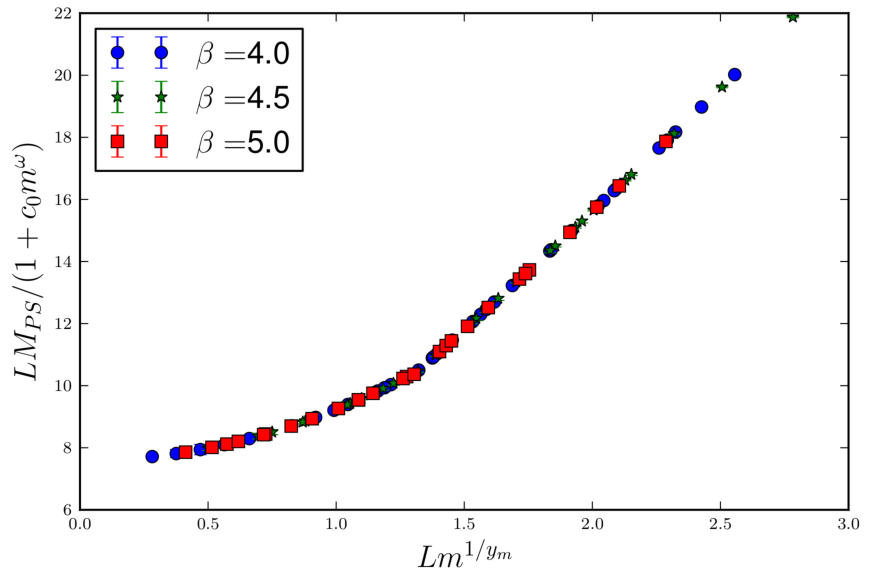
\includegraphics[width=0.45\linewidth]{pion_combined}\hfill
  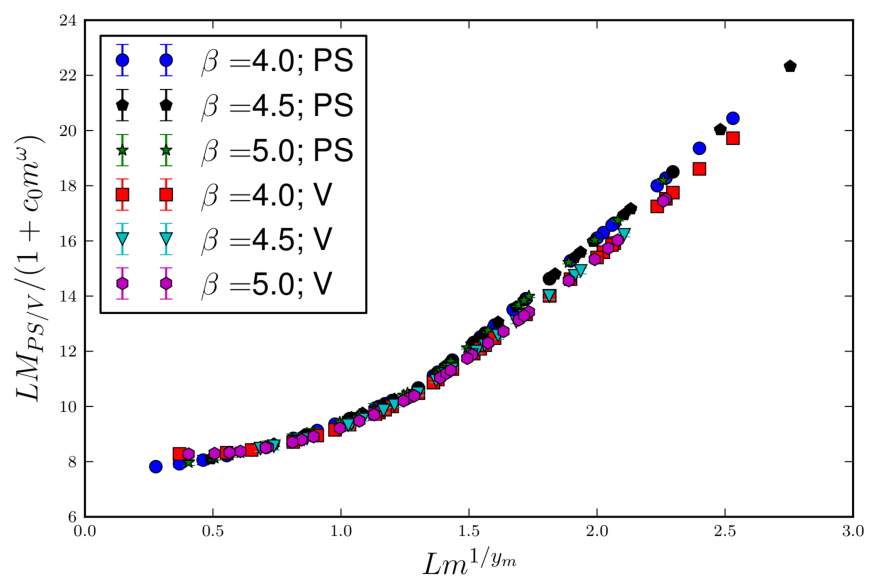
\includegraphics[width=0.45\linewidth]{rho_combined}
  \caption{\label{fig:fss_combined} Left panel: The best curve collapse fit for the pseudoscalar mass combining  all available gauge couplings, including the published data of Ref.~\protect\cite{Fodor:2011tu,Aoki:2012eq}. The fit parameters are listed in Table~\protect\ref{table:results}. Right panel: Similar fit combining the pseudo scalar and  vector meson masses and $f_\pi$.  }
\end{figure*}
%%%%%%%%%%%%%%%%%%%%%%%%%%%%%%%%%

We can significantly strengthen  the finite size scaling fit   by combining data at different gauge couplings. If the gauge coupling is an irrelevant operator the scaling function $F_H(x)$ should be independent of $\beta_F$. Such a global fit allows us to determine both  scaling dimensions  $y_m$ and $y_0$. The fit also depends on the  scaling function $F_H(x)$ that is  independent of $\beta_F$, and the coefficients $c_0$ that depend on the gauge coupling. In addition we need a new parameter $s_m$ that rescales the bare mass $m \to s_m m$ to a common reference value. In the following we choose $s_m=1$ at $\beta_F=4.0$. $s_m$ depends on the gauge coupling but is independent of the operator. The next entry in Table~\ref{table:results} lists the results of a fit to the pseudo scalar mass that combines $\beta_F=4.0$, 4.5 and 5.0. We use the same  form of two quadratic polynomials to fit the data and minimize the $\chi^2$ using a Bayesian fitter. \TODO{Yuzhi, do you want to add a sentence about the fit and fitter and a reference?}  The universal fit parameters $y_m$ and $y_0$ are consistent with previous values with $\chi^2$/dof  comparable to the   $\beta_F=4.0$ one. Including  data sets at $\beta_F=2.8$, 5.5 and 6.0 does not change the conclusion. As expected the  scale factors $s_m$ increase with decreasing $\beta_F$ but the $c_0$ coefficients decrease, suggesting that the conformal infrared fixed point with $g_0\approx 0$ occurs at weaker gauge coupling. 

If the gauge coupling is an irrelevant operator, one should be able to combine different lattice actions, not only different gauge couplings. Both the LHC and Lat-KMI collaborations ~\protect\cite{Fodor:2011tu,Aoki:2012eq} published their spectrum results which we combine with our data. As the  next entry of Table~\ref{table:results} shows, such a combined fit with 191 independent degrees of freedom is possible and results in $\chi^2$/dof=1.2.  The left panel of \fig{fig:fss_combined} illustrates the curve collapse of this fit. 

Until now we considered only the pseudo scalar mass. The vector meson mass and $f_\pi$ can be analyzed similarly, one can even combine the three operators. The fit now depends on the universal scaling dimensions  $y_m$ and $y_0$, three scaling functions $F_H(x)$ for the three operators, the scale factors $s_m$ at each gauge coupling value and the $c_0$ coefficients that depend both on the operator and $\beta_F$. 
\TODO{ We might fix sm from the pion and reduce parameters other ways as well. This is still to be done!} 
\TODO{Add Nf=8; interpret and conclude} 


% ------------------------------------------------------------------
\section{Conclusion}
\TODO{This is from the Pos} We have demonstrated that apparent inconsistencies in finite size scaling analyses of the $N_f=12$ system can be resolved by considering the effect of the leading irrelevant gauge coupling, at least for $f_\pi$ and the pseudoscalar and vector meson masses.
We find that all three quantities, when considered independently, prefer an anomalous dimension $\gamma_m^{\star} = y_m^{\star} - 1 \approx 0.25$.
By performing a combined fit to all data used in this work, we hope to strengthen our conclusion and obtain a robust prediction for $\gamma_m^{\star}$.
It will also be important to consider other quantities, such as the string tension and mass of the lightest baryon, but at present we do not have these data available to analyze.

We expect that systems near the conformal boundary will generically possess a nearly-marginal gauge coupling.
The initial results presented here suggest that this may have important effects that will need to be investigated in future studies of strongly-coupled many-flavor systems.
% ------------------------------------------------------------------


Finite size scaling techniques provide an effective tool to investigate models governed by a fixed point with only one relevant operator, especially if the irrelevant operators are strongly irrelevant, i.e., their scaling dimensions are much below zero.
If this condition is not met, either very large volumes have to be used, or corrections to scaling have to be taken into account.
Both perturbation theory and non-perturbative step scaling function calculations predict that in the 12-flavor systems the gauge coupling has very small scaling exponent, $-0.3 \lsim y_0 \lsim -0.1$~\cite{Ryttov:2010iz, Appelquist:2009ty}.
In this paper we consider the possibility that some of the inconsistencies found in earlier investigations are due to this nearly-marginal gauge coupling.

In order to investigate the effects of a nearly-marginal irrelevant gauge operator, it is essential to study the system at many gauge coupling values.
In this work we cover a wide range from a strong coupling near the onset of the ``$\Sb$'' lattice phase~\cite{Cheng:2011ic} to as weak coupling as our lattice volumes allow.
We find that finite size scaling using only the leading relevant operator predicts scaling exponents that depend both on the physical quantity considered as well as on the bare gauge coupling, as shown in the left panel of \fig{fig:scaling_exp}.
When we include the corrections to scaling due to the nearly-marginal gauge coupling, our preliminary analysis predicts scaling exponents that are, within errors, independent of the gauge coupling and consistent for the pseudoscalar meson, vector meson, and $f_\pi$, as shown in the right panel of \fig{fig:scaling_exp}.

While we cannot prove that all physical quantities will scale consistently once corrections to scaling are taken into account -- especially because these corrections might be more important to some quantities than to others -- our results resolve some of the existing controversies of the 12-flavor system and reinforce the IR-conformal interpretation suggested by our earlier studies of the bare step scaling function~\cite{Hasenfratz:2011xn}, phase transitions~\cite{Hasenfratz:2013uha} and Dirac eigenvalues~\cite{Cheng:2013eu}.
Our finite size scaling results prefer a fairly small anomalous dimension, $\gamma_m^{\star} = y_m^{\star} - 1 \approx 0.25$.
The statistical errors on $\gamma_m^{\star}$ are about 10\%, with similar systematic uncertainties for the three quantities considered.
At this point we cannot give a more precise error estimate, but note that this value is consistent with our findings for $\gamma_m^{\star}$ from the Dirac operator spectral density~\cite{Cheng:2013eu}.
% ------------------------------------------------------------------


% ------------------------------------------------------------------
\section*{Acknowledgments} % Draft complete
We thank Julius Kuti for his helpful probing questions, Biagio Lucini for suggesting that we include corrections to finite-size scaling, and Roman Zwicky for useful discussions concerning the correction terms.
Part of this work was performed when A.~H.\ and D.~S.\ visited the Aspen Center for Physics (NSF Grant No.~1066293) and CP$^3$-Origins in Odense, and we thank both institutions for their support and hospitality. A.~H. is grateful for the hospitality of the Brookhaven National Laboratory HET group during her extended visit.
This research was partially supported by the U.S.~Department of Energy (DOE) through Grant No.~DE-SC0010005 (A.~C., A.~H.\ and D.~S.) and by the DOE Office of Science Graduate Fellowship Program under Contract No.~DE-AC05-06OR23100 (G.~P.).
Our code is based in part on the MILC Collaboration's public lattice gauge theory software.\footnote{\texttt{http://www.physics.utah.edu/$\sim$detar/milc/}}
Numerical calculations were carried out on the HEP-TH and Janus clusters at the University of Colorado; at Fermilab under the auspices of USQCD supported by the DOE; and at the San Diego Computing Center through XSEDE supported by National Science Foundation Grant No.~OCI-1053575.
% ------------------------------------------------------------------



% ------------------------------------------------------------------
{\renewcommand{\baselinestretch}{0.86} % Decreases spacing between lines
  \bibliography{fss}
  \bibliographystyle{apsrev}
}
\end{document}
% ------------------------------------------------------------------
